\vssub
\subsubsection{~Triangular unstructured grids} \label{sub:num_space_tri}
\conthead{WWM-II}{A. Roland, F. Ardhuin, M. Dutour-Sikiri\'c, A. Abdolali}

\noindent
Triangle-based unstructured grids can be chosen in \ws\ by using
numerical schemes based on contour residual distribution (CRD)
\citep{art:ricchiuto2005} for the discretization of the space
derivative. These schemes have been adopted to the wave action
balance equation in \citep{rep:Roland2008} and have been
implemented in the Wind Wave Model-II (WWM-II) and in WW-III.
With respect to the time integration methods, explicit
and implicit schemes are available for unstructured grids.
If the explicit solver is chosen the original fractional step
method of WW3 is used, where the solution of the two dimensional
hyperbolic part in geographical space is solved on unstructured
grids based on the above mentioned methods. In this case the
spectral part and the source terms are integrated in a similar
way as in the structured version of WW3. The definition of the time
steps is also done in the same way as for the structured part except
that the number of sub-iterations for the unstructured part are estimated
automatically based on the maximal CFL number in the domain. If implicit methods
are chosen, a linear equation system is assembled based
on the CRD-N schemes following \citep{rep:Roland2008}.
The spectral propagation part is solved with simple implicit
1$^{st}$ order upwind schemes and the source terms are written  in
the matrix in the same way as in the dynamic
scheme of WW3 using $\epsilon = 1$ in eq. 3.61 and assembling the
equation system following simple Patankar rules. The full description of new implementations is discussed in \cite{rolandetal2019t}
It can be shown analytically and by numerical experiment that
for CFL \textless 1 the explicit and the implicit methods give similar results.
This was also demonstrated in practical applications
e.g. \citep{rep:Abdolalli2018, Smith2018, rep:Abdolalli2019, AbdolaliEtAl2019OM}. However, for CFL \textgreater 1
the transient solutions of the implicit schemes
have a time step depedency since the source terms are linearized
in time. The time step in the implicit schemes is equal the global timestep
and the other time steps for spectral space or source terms have no effect.
The fractional step methods has a time step
dependency as well due to the splitting errors, which become
especially predominant in shallow water \citep{rep:Roland2008}.
For both numerical methods proper convergence analysis with respect
to the global time step and the spatial resolution
need to be carried out unless the level of accuracy is
satisfactory for the given applications. The numerical implementations
have subsequently been evaluated in WWIII \citep[e.g.][]{art:Aea09,art:babanin2011,art:bertin2014,
art:bertin2015,art:dodet2013,art:ferrarin2008,art:ferrarin2013,art:janekovic2015,art:kerr2013,art:liau2011,art:Mea10,art:perrie2018,
art:perrie2013two,pro:rol2006a,pro:rol2006b,art:rol2009,art:rol2012,art:rol2014,art:sikiric2012,art:sikiric2013,art:sikiric2018,
pro:zanke2006}.


This option is activated by setting the grid string to `{\code
UNST}' in {\file ww3\_grid.inp}.  Four schemes have been implemented, and the
choice of one or the other is done with the {\code UNST} namelist.  These are
the CRD-N-scheme (1st order), the CRD-PSI-scheme (better than 1st order, 2nd
order on triangular structured grids), the CRD-FCT-scheme (2nd order
space-time), and the implicit N-scheme. The default is the most efficient but
diffusive explicit N-scheme. An implicit variant of the RD-Schemes
using the method of lines and the N-Scheme for the space discretization was
implemented in the SWAN model by \cite{art:Zij10}  a similar discretization
is chosen in the actual version of ECWAM see \cite{pro:rol2012}.

In this method the evolution of the spectrum at the nodes, where it is
evaluated, is based on the redistribution over the nodes of the flux
convergence into the median dual cells associated with the nodes (see Figure
\ref{fig:triangles}).  For any spectral component, the advection equation, Eq.
(\ref{eq:step_xy_prop}), is solved on the median dual cells: the incoming flux
into a cell gives the rate of change of the wave action at the corresponding
node. The various schemes implemented have different discretization for the
estimation of this flux. The schemes have been presented in \citep[see][for a
review]{rep:Roland2008}.

We note that these advection schemes do not include corrections for
the garden sprinkler effect (GSE). In the usual sense of GSE corrections
it was found that the N-Scheme has sufficient numerical cross-diffusion
to well compensate for this effect. However, higher order schemes such
as CRD-PSI or CRD-FCT may create significant GSE effecting depending
on the spatial resolution.

The parallelization of the unstructured grid schemes is done either
using the Card Deck approach, as done for the structured grids, or using
domain decomposition methods. The domain decompositions methods are based
on ParMetis \citep{rep:karypis2011metis}, which is a C implementation of a parallel
graph partitioning algorithm. ParMetis is being interfaced using
PDLIB (Parallel Decomposition Library) in Fortran, which beside interfacing
ParMetis provides the needed exchange routines for unstructured
grids using the Fortran2002 standard. The exchange routines do
all the needed communication for the decomposed grids between the
various threads based on the decomposition provided by ParMetis.
In this way, all the domain decomposition parts are incorporated in
the main source with just one line of code. For the compilation of
the PDLIB option in the switch files, which activates the domain
decomposition parallelization, ParMetis needs to be installed
and the code needs to be compiled with using MPI. PDLIB works with
all usual MPI implementations, such as OpenMPI or MPICH2 and others. An schematic view of implemented parallelization algorthims in WW3 (card deck and domain decomposition) are shown in figure \ref{DDvsCD}. For real case applications, the convergence of these two methods is demonstrated in \cite{AbdolaliEtAl2019OM} for Hurricane Ike, 2008.

In practice, the unstructured grid can be easily generated, using the PolyMesh
software (developed by Aron Roland), from a shoreline polygons database
and a list of arbitrary depth soundings. PolyMesh interfaces Triangle and adopts
a-priori error estimates based on wave propagation characteristics and depth error
based on the barycentric bathymetric error \citep[e.g.][]{art:WS96}. 
Other grid generation tools such as SMS and OceanMesh2D can also be used. There
are no constrains with respect to the triangle shape.

The equivalent of the CFL condition for explicit finite difference schemes
on regular grids is the ratio of the dual cell area divided by the product
of the time step and the sum of the positive fluctuations into the dual cell.
Because the spectral levels are imposed on the boundary
for the positive fluxes, the boundary nodes are excluded from this CFL
calculation and the incoming energy is set to zero, whereas the outgoing energy
is fully absorbed. Only for the reflection part energy is allowed to penetrate
from the boundary into the domain.

The boundary condition at the shoreline depends on the wave direction
relative to the shoreline orientation. This particular treatment is enforced
using the `{\code IOBPD}' array which is updated whenever the grid points
status map `{\code MAPSTA}' changes. The grid geometry is also used to define
local gradients of the water depth and currents. All other operations, such as
interpolation of the forcing on the grid and interpolation from the grid onto
output locations, is performed using linear interpolation in triangles.

All the triangle geometry operations assume a locally flat Earth. Depth and
current gradients on the grid are estimated at the nodes by interpolating
within on triangle using linear shape functions.

\begin{figure} \begin{center}
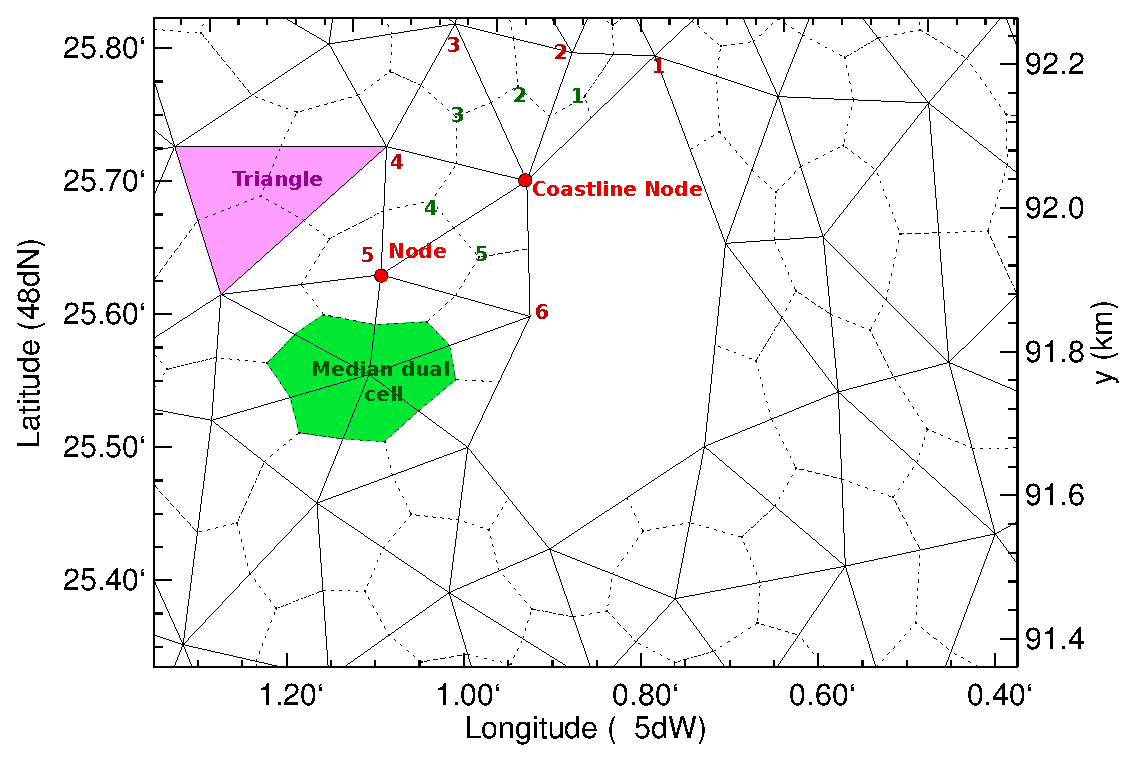
\epsfig{file=./num/grid_triangles.eps,angle=0,width=4.in}
\caption{Example of a region of a triangle-based mesh, with in this case the
 small Island of Bannec, France. If the depth is greater than the minimum
depth, the nodes of the shoreline are active. These are characterized by a
larger number of neighbor nodes (6 in the example chosen) than neighbor
triangles (5 in the same example).}
\label{fig:triangles} \botline
\end{center}
\end{figure}


\begin{figure} \begin{center}
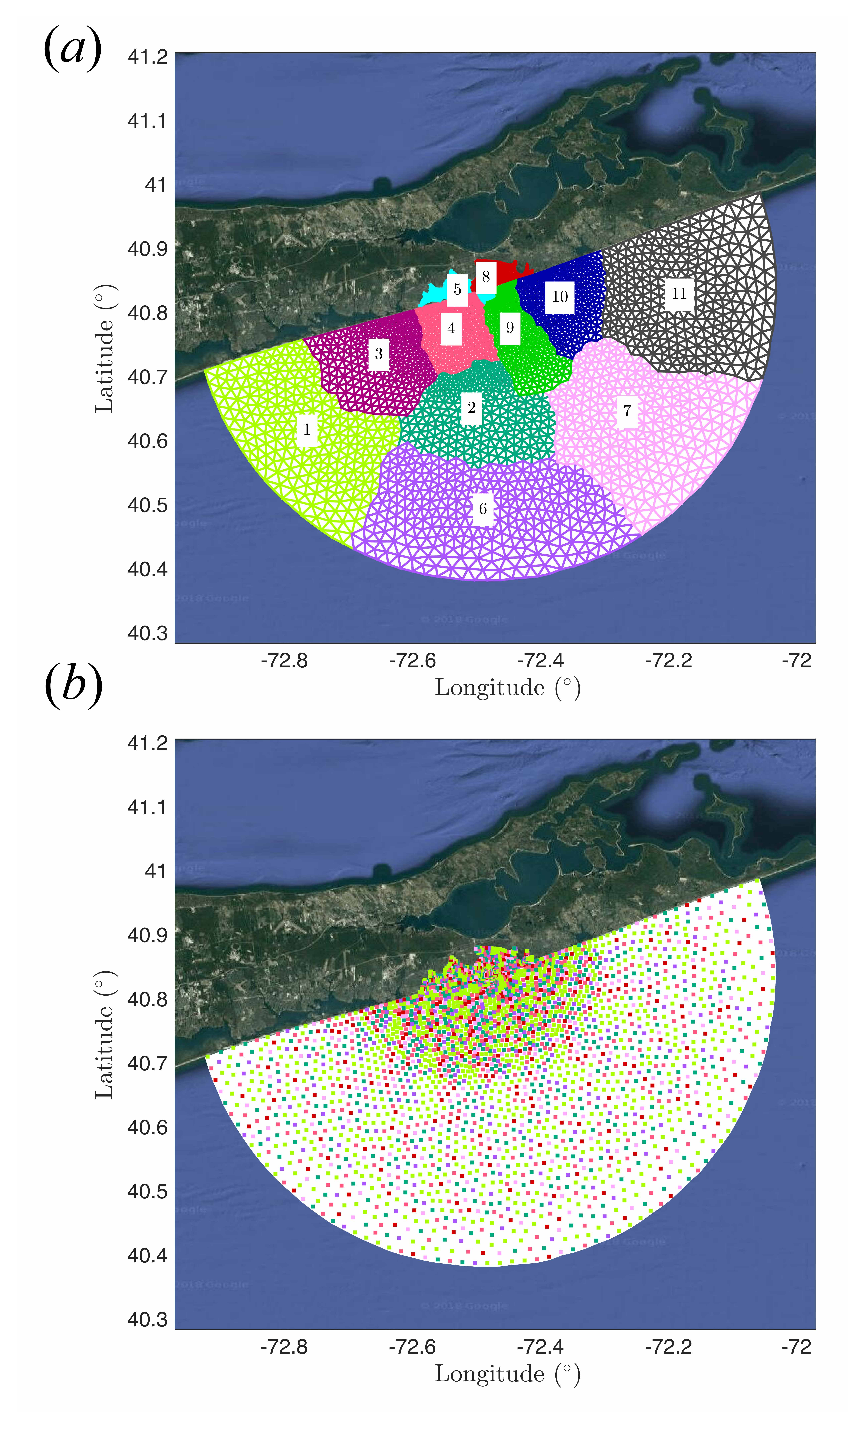
\epsfig{file=./num/DDvsCD.eps,angle=0,width=4.in}
\caption{The schematic difference between Domain Decomposition (a) and Card Deck approach (b) on 11 computational cores represented by colors. The grid has $\sim$3k nodes  and is build for Shinnecock Inlet, NY taken from an ADCIRC example problem.}
\label{DDvsCD} \botline
\end{center}
\end{figure}

